\begin{frame}[t]
    \frametitle{Results: Canonical refining}
    \framesubtitle{Discovering \textit{de-novo} miRNAs}
    \begin{figure}[h!]
        \centering
        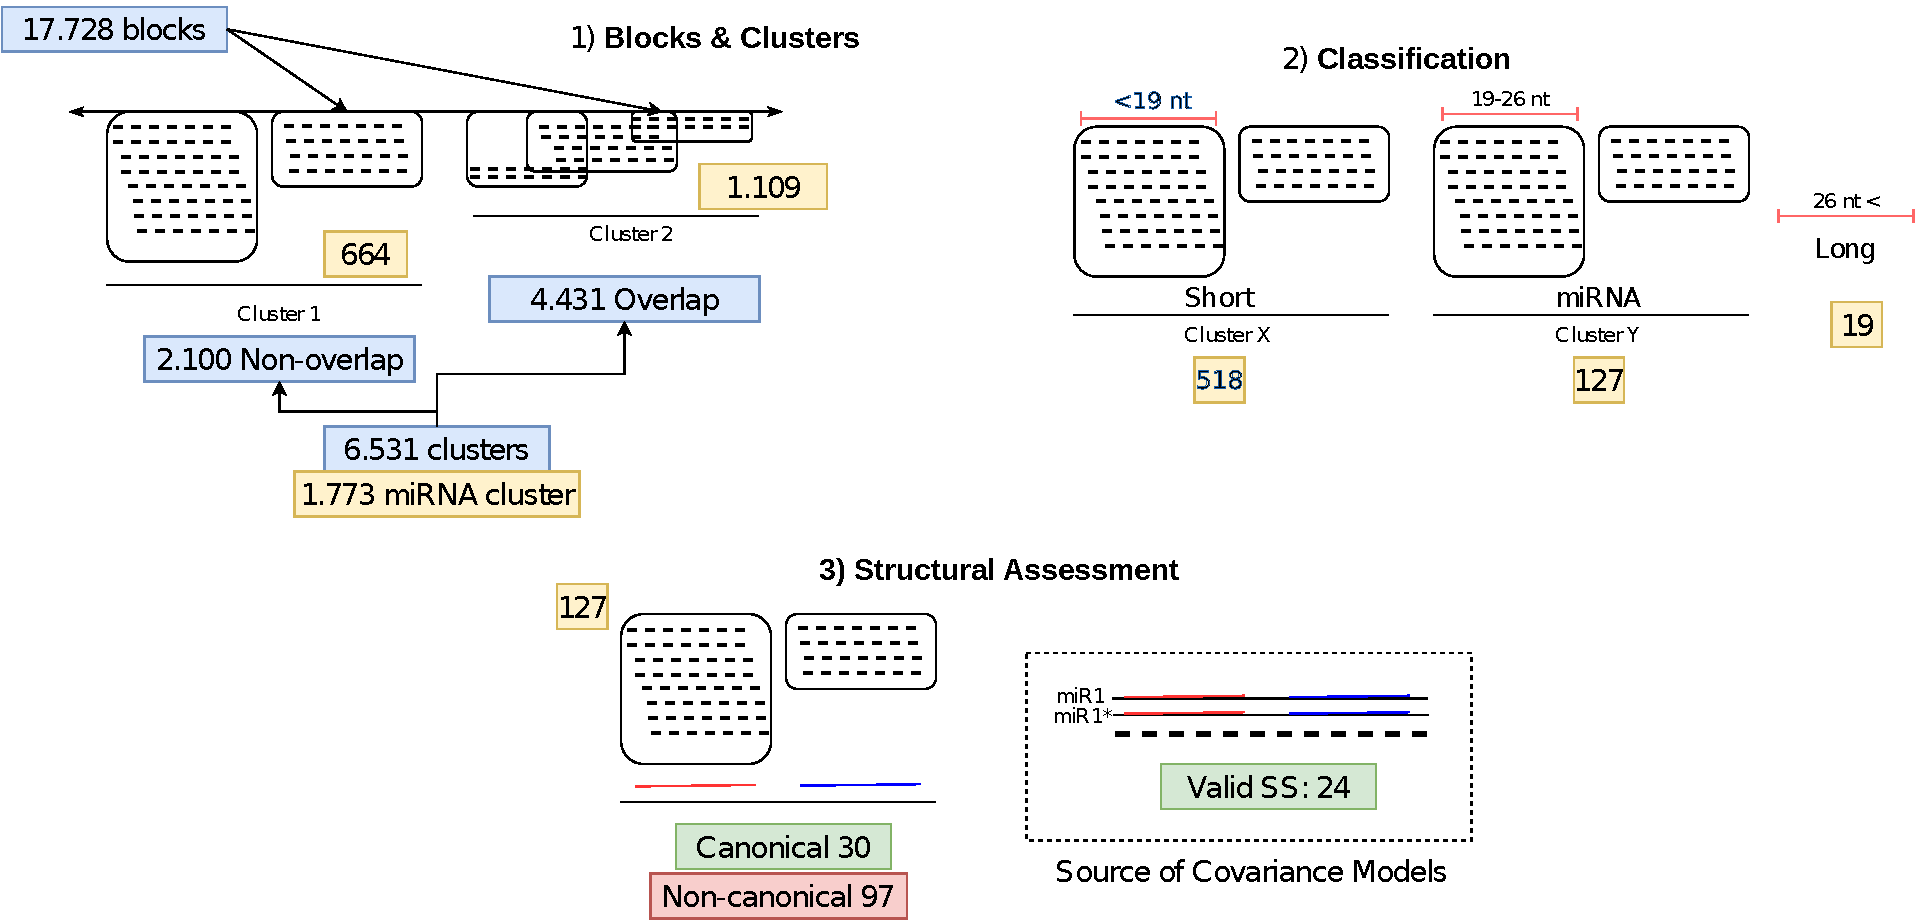
\includegraphics[width=\linewidth]{Figures/results_workflowALL}\label{fig:workflow} %
    \end{figure}
    \begin{itemize}
        \item[-] Only $3.6$\% candidates detected as \textit{canonical} miRNAs.
        \item[-] Most of candidates detected as piwi-RNAs ($\sim 77.4$\%)
    \end{itemize}
\end{frame}

\begin{frame}[t]
    % Take the most expressed candidates from the 24 ones and show one comparison.
    \frametitle{Results: Going back to Chr7 cluster}
    Canonical de-novo families: One additional candidate on Chr7 $:($
    \begin{figure}[h!]
        \centering
        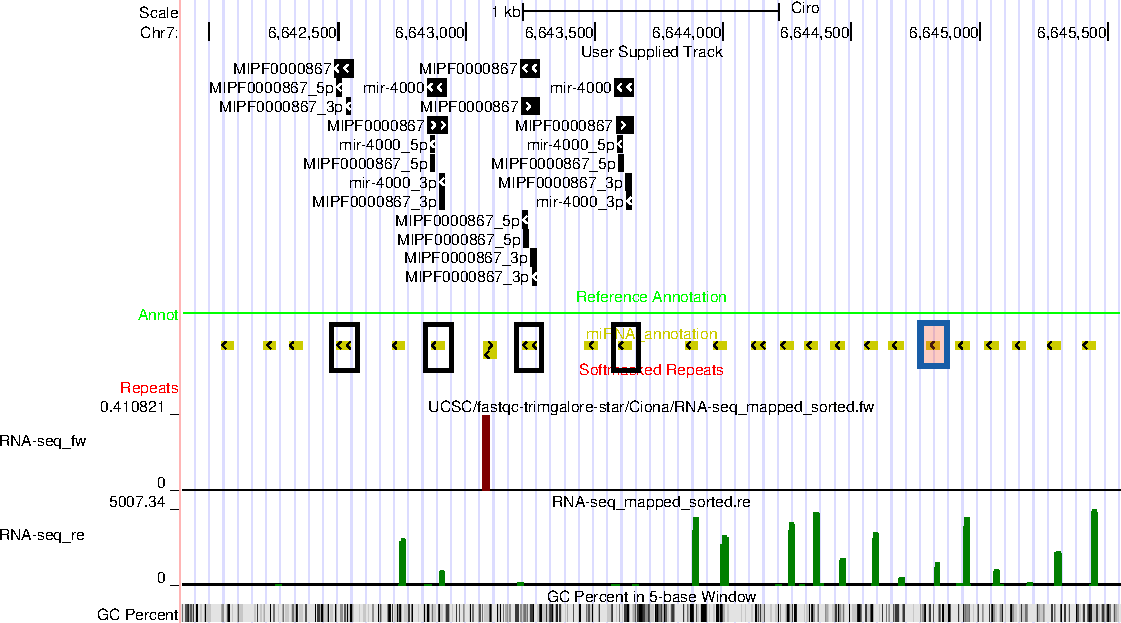
\includegraphics[width=0.9\linewidth]{Figures/homology_coverage_denonvo} %
    \end{figure}
    \textbf{Why $\sim82$\% loci were not detected?} 
\end{frame}

\begin{frame}[t]
    % Take the most expressed candidates from the 24 ones and show one comparison.
    \frametitle{Results: miRNA annotation on chordates}
    \begin{figure}[h!]
        \centering
        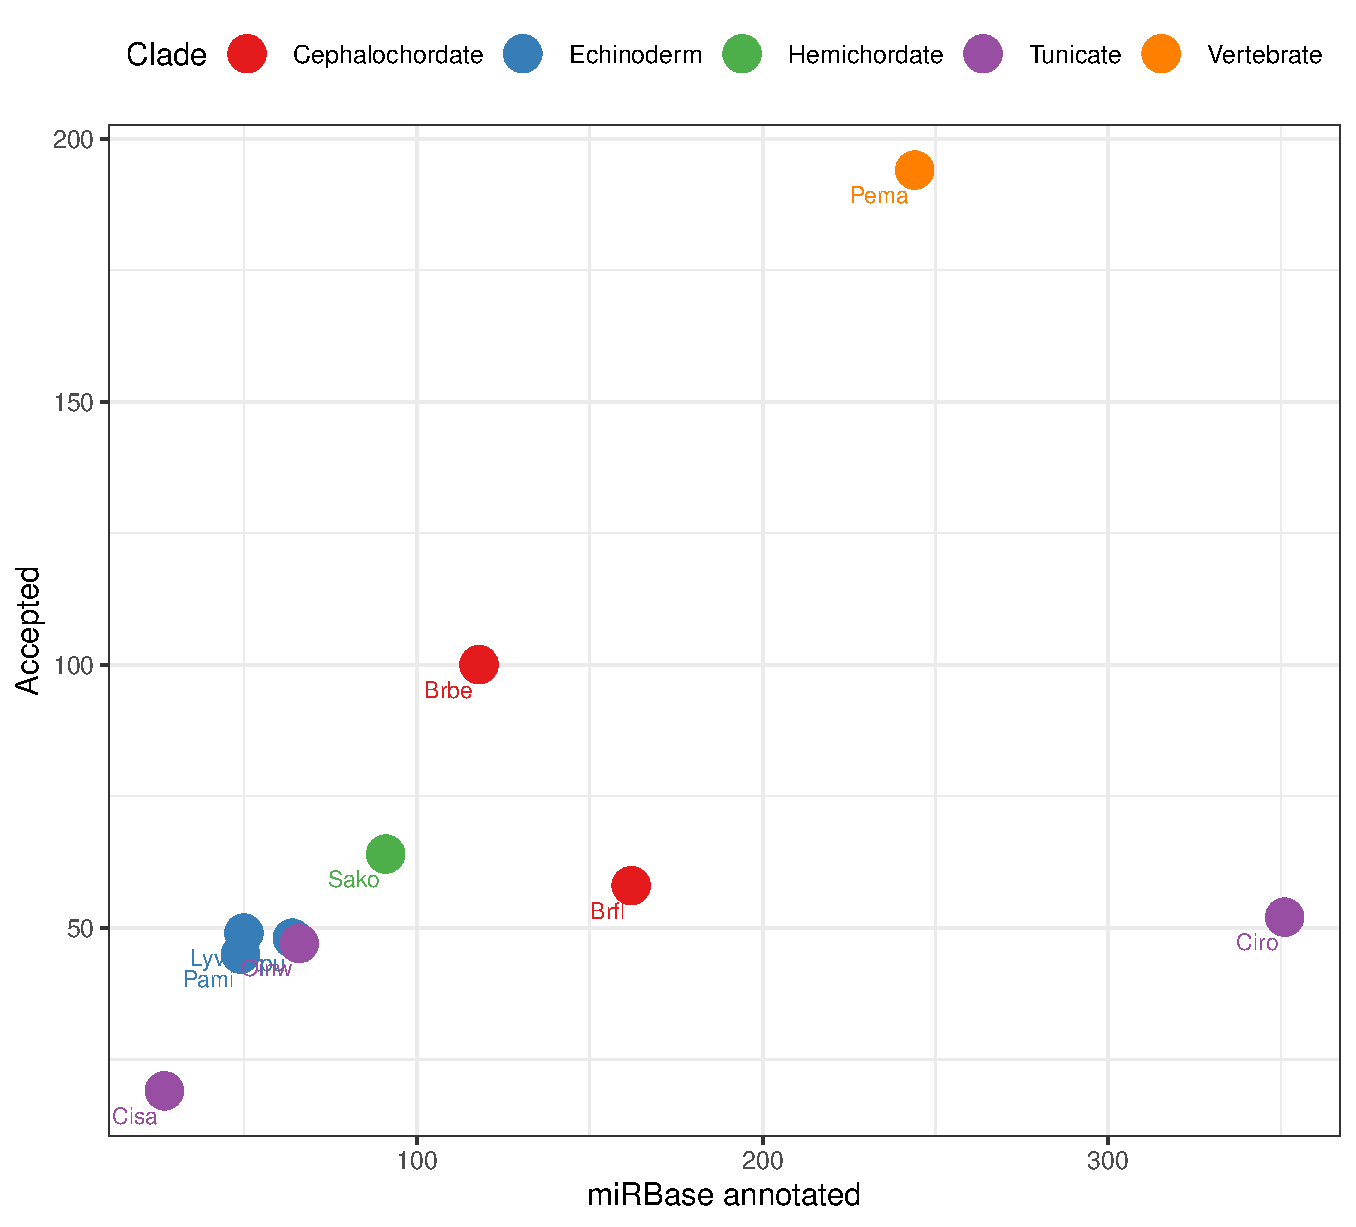
\includegraphics[width=.45\linewidth]{Figures/annotated_vs_accepted} %
    \end{figure}
    \begin{itemize}[<+->]
        \item \textit{C.\ robusta} annotations: $351$ loci
        \item With Fam.: $18.5$\% / No Fam: $81.5$\%.
        \item $13\times$ than sister specie: \textit{Ciona savignyi}
        \item Higher loci number than coelacanth and lancelet (!).
    \end{itemize}
\end{frame}

\begin{frame}[t]
    % Take the most expressed candidates from the 24 ones and show one comparison.
    \frametitle{Results: Discovering canonical miRNAs}
    Finding canonical de-novo families: Structural assessment
    \begin{figure}[h!]
        \centering
        \includegraphics<1>[width=\linewidth]{Figures/evaluation_annotation_mirbase1} %
        \includegraphics<2>[width=\linewidth]{Figures/evaluation_annotation_mirbase2} %
    \end{figure}
     \begin{itemize}[<+->]
         \item Canonical miRNAs represent $\sim21$\% of cluster.
         \item Reasons: Position of mature sequences, loop regions, structural constrains.
     \end{itemize}
\end{frame}

%\begin{frame}[t]
%    \frametitle{Results: Iteration $1$}
%    \framesubtitle{Discovering \textit{de-novo} miRNAs}
%    \begin{itemize}
%        \item Starting point: $24$ CMs from \textit{C.\ robusta}.
%        \item First target specie: \textit{Ciona savignyi}.
%    \end{itemize}
%\end{frame}
